\section{Markov chains}
\label{sec:markovchains}

We introduce here the concept of Markov chains and show it relations
with FSMs.

\subsection{Definition}

A (discrete-time) Markov chain is a stochastic process for which the
joint distribution of $N$ consecutive samples
$\Matrix{z} = (z_1, \dots, z_N)^\top$ factorizes as:
\begin{align}
    p(\Matrix{z}) &= p(z_1)\prod_{i=2}^n p(z_i | z_{i-1}),
    \label{eq:markovchains:infinite_markovchain}
\end{align}
where $p(z_1)$ is the \emph{initial probability} and $p(z_i | z_{i-1})$
is the \emph{transition probability}. Let's consider a slightly revise
definition of this stochastic process: let suppose that, in order to
observe a sequence $\mathbf{z}$ the stochastic process has to halt
for an instant. Let's assume further that the probability of halting
depends on the state. The process can halt when certain states are
drawn but not for some other states. Noting $p(\emptyset | z_n)$ the
probability of halting when in state $z_n$, the probability of
observing a sequence becomes:
\begin{align}
    p(\mathbf{z}) &= p(z_1) p(\emptyset | z_n) \prod_{i=2}^n p(z_i | z_i-1)
    \label{eq:markovchains:finite_markovchain}
\end{align}

\subsection{FSM representation}

Equation \ref{eq:markovchains:finite_markovchain} can be very
naturally mapped to a $d$-state FSM using the probability semiring with:
\begin{align}
    \boldsymbol{\alpha} &= \begin{bmatrix}
        p(z_1 = 1) \\
        \vdots \\
        p(z_1 = d)
    \end{bmatrix} \\
    \mathbf{T} &= \begin{bmatrix}
        p(z_i = 1 | z_{i-1} = 1)  & \dots & p(z_i = d | z_{i-1} = 1) \\
        \vdots  & \ddots & \vdots \\
        p(z_i = 1 | z_{i-1} = d)  & \dots & p(z_i = d | z_{i-1} = d) \\
    \end{bmatrix} \\
    \boldsymbol{\omega} &= \begin{bmatrix}
        p(\emptyset | z_1 = 1) \\
        \vdots \\
        p(\emptyset | z_1 = d)
    \end{bmatrix}.
\end{align}
The states'label is application dependent and can be defined in many
ways.

\paragraph{} The relation between the Markov chains and FSM brings many
advantages, notably:
\begin{itemize}
    \item the constructive operations (union, concatenation,
        composition, ...) allow to create easily complex distribution
        over sequences
    \item several important inference algorithms can be seen as special
        instance of the total sum algorithm, there are therefore easily
        implemented and optimized.
\end{itemize}

\subsection{Inference algorithms}

The use Markov chains in machine learning problem usually necessitate
to solve two inference problem: (i) state-marginalization and (ii)
calculate the probability of the most likely sequence. We show how this
two algorithms can be calculated easily using the FSM formalism.

\subsubsection{State marginalization}
We aim to calculate the following
quantity:
\begin{align}
    p(z_i) &= \sum_{z_1, \dots, z_{n}} p(z_1, \dots, z_{i-1}, z_i, \dots, z_n) \\
    &= \sum_{z_{i-1}} p(z_i | z_{i-1}) p(z_{i-1}).
    \label{eq:markovchains:statemarginal}
\end{align}
Equation \ref{eq:markovchains:statemarginal} leads to a recursive
function which is trivially evaluated with the total sum algorithm:
\begin{align}
    \mathbf{v}_i &= \begin{bmatrix}
        p(z_i = 1) \\
        \vdots \\
        p(z_i = d)
    \end{bmatrix} = \mathbf{T}^\top \mathbf{v}_{i-1}
    \label{eq:markovchains:totalsum_statemarginal}
\end{align}
with initial condition $\mathbf{v}_1 = \boldsymbol{\alpha}$.

\paragraph{} In practice, \eqref{eq:markovchains:totalsum_statemarginal} is not
numerically stable as it multiplies many numbers smaller than ones
leading to numerical underflow  of floating point arithmetic. However,
this issue is easily solved by taking the logarithm of all values of
$\mathbf{T}$  and $\mathbf{v}_i$ and using the log-semiring.

\paragraph{} This computation is at the heart of the forward-backward algorithm
used to train Hidden Markov Models and to compute the gradient of
several sequence-discriminative objective function.

\subsubsection{Best path probability}

We aim to find:
\begin{align}
    \max_{z_1, \dots, z_{n}} p(\mathbf{z}) = \max_{z_{i+1}, \dots, z_n} p(z_{i+1}, \dots, z_n)
\end{align}

Whereas the graph conveniently represents the possible trajectories in
the state-space, the transition matrix $\Matrix{T}$ allows to express
state marginalization as a matrix-vector multiplication. For instance:
\begin{align}
    p(z_n) &= \sum_{i \in \{a, b, c\} } p(z_{n-1}=i, z_n) \\
    &= \sum_{i \in \{a, b, c\}} p(z_n | z_{n-1} = i) p(z_{n-1} = i) \\
    \Matrix{v}_n &= \Matrix{T} \Matrix{v}_{n-1} \label{markovchains:eq:smarginal}
\end{align},
where:
\begin{align}
    \Matrix{v}_n &= \begin{bmatrix}
        p(z_n = a) \\
        p(z_n = b) \\
        p(z_n = c)
\end{bmatrix}.
\end{align}

Equation \eqref{markovchains:eq:smarginal} is the ``core'' operation of many
Markov chains related algorithm such as forward-backward (for training models)
and viterbi (for decoding speech). For Markov chains that have a large number
of states, this operation is problematic as its complexity is quadratic in the
number of states: $\mathcal{O}(2D^2)$ where $D$ is the number of states.
The rest of the document describes how to exploit the structure of the Markov
chains to decrease the complexity of this operation.

\subsection{Compact graphical form}
In many application, the transition probabilities have some structure
allowing to represent the Markov chain in a more compact manner. For
instance, let's consider the following transition probabilities:
\begin{align}
    p(z_n = j | z_{n-1} = i) &= \begin{cases}
        \gamma + \nu_i \delta_j & \text{if } i = a \text{ and } j=b \\
        \nu_i\delta_j & \text{otherwise}.
    \end{cases}
\end{align}
Defined in this way, this Markov chain has $2 \cdot 3 + 1 = 7$
parameters instead of $3 \cdot 3 = 9$ in the general case. The graphical
representation of this constrained Markov chain is shown in
Fig.~\ref{markovchains:fig:consgraph}.
%
\begin{figure}[t]
    \centering
    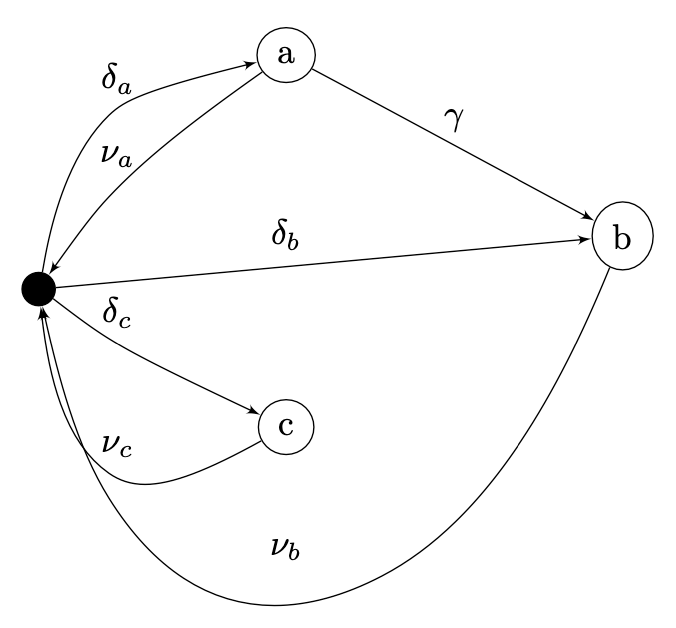
\includegraphics[scale=0.5]{images/consgraph_resized.png}
    \caption{Graphical representation of a constrained Markov chain.
    The filled node is a ``phony'' state equivalent of the
    \emph{epsilon-arc} in the WFST framework.}
    \label{markovchains:fig:consgraph}
\end{figure}

\subsection{Efficient marginalization}

In many applications, we would like to use the structure of the Markov
chain to efficiently marginalize over a state. The formula in
\eqref{markovchains:eq:smarginal} can be prohibitive to evaluate if the
state-space is large. The idea is to use the constraints of the Markov
chain to efficiently calculate the matrix-vector product.


In our particular example, observe that the transition matrix can be
written as:
\begin{align}
    \Matrix{T} &= \Matrix{S} + \Matrix{\nu} \Matrix{\delta}^\top,
\end{align}
where:
\begin{align}
    \Matrix{S} &= \begin{bmatrix}
        0 & \gamma & 0 \\
        0 & 0 & 0 \\
        0 & 0 & 0
    \end{bmatrix} \;
    \Matrix{\nu} = \begin{bmatrix} \nu_a \\ \nu_b \\ \nu_c \end{bmatrix}\;
    \Matrix{\delta} = \begin{bmatrix} \delta_a \\ \delta_b \\ \delta_c \end{bmatrix}.
\end{align}
Consequently, we have:
\begin{align}
    \Matrix{T} \Matrix{v}_{n-1} &= (\Matrix{S} +
        \Matrix{\nu} \Matrix{\delta}^\top) \Matrix{v}_{n-1},
\end{align}
and using the associativity and the distributive properties of the addition and
multiplication we re-write it as:
\begin{align}
    \Matrix{T} \Matrix{v}_{n-1} &= \Matrix{S} \Matrix{v}_{n-1} +
        \Matrix{\nu} (\Matrix{\delta}^\top \Matrix{v}_{n-1}) \label{markovchains:eq:fast_smarginal}.
\end{align}
Calculating the matrix-vector product following the operation order of
\eqref{markovchains:eq:fast_smarginal}, the complexity reduces to:
$\mathcal{O}(2Q + 2D)$ where $Q$ is the number of non-zero elements in
$\mathbf{S}$.

\paragraph{Remark:} in the general case, it is easy to show that:
\begin{align}
    \Matrix{T} &= \Matrix{S} + \sum_{k}^K \Matrix{\nu}_k \Matrix{\delta}_k^\top,
    \label{markovchains:eq:tfactor}
\end{align}
where $K$ is the number of ``phony'' states in the graphical representation
of the Markov chain\footnote{
    Here, I assume that there is no looping path starting from a ``phony''
    state that does not contain a ``real'' state. This constraint
    is necessarly met in practice.
}\footnote{
    The factorization in \eqref{markovchains:eq:tfactor} is not unique.
}.

\end{document}

